\chapter{Modelli di Fonti Luminose e Superfici}
\section{Modellazione di Superfici}
\begin{figure}[tb]
	\centering
	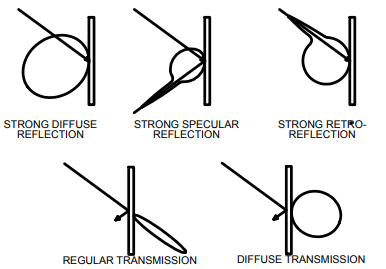
\includegraphics[width=0.4\linewidth]{../assets/chapter3_surfaces_interaction_types.png}
	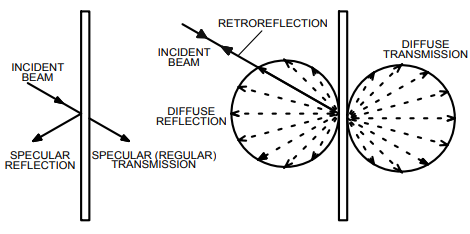
\includegraphics[width=0.4\linewidth]{../assets/chapter3_surfaces_specular_interaction.png}
	\caption{tipi di riflessione e trasmissione. Immagine da \cite{art-rad}}
	\label{chapter3:surface:interactionTypes}
\end{figure}
Quando un flusso radiante incide su una superficie, i tre processi che avvengono sono \textit{riflessione}, \textit{trasmissione}, 
\textit{assorbimento}, oltre all'emissione per tutti i materiali al di sopra dello zero assoluto. 
In particolare, durante la propagazione di un flusso radiante in un mezzo, parte della sua energia viene assorbita o 
deviata dal mezzo\footnote{d'ora in poi in questo capitolo si trascura la propagazione nel mezzo e si considera propagazione nel vuoto}.
Quando la luce incontra un oggetto, in particolare la sua superficie esterna, detta \textit{interfaccia}, tale flusso radiante pu\`o essere 
trasmesso e/o riflesso in diverse direzioni e con diversa intensit\`a.\par
Per il principio di conservazione dell'energia, all'interfaccia deve valere la propriet\`a\footnote{notazione introdotta in seguito}
\begin{equation}\label{chapter3:surface:interfaceEnergyConservation}
	\bar{\rho} + \bar{\uptau} = 1
\end{equation}
Si noti l'assenza del coefficiente di assorbimento, in quanto esso non \`e rilevante nell'interazione luce-interfaccia, ma partecipa in processi che 
coinvolgono la propagazione all'interno del volume del materiale, nel quale vale, per ogni lunghezza d'onda, in ogni istante, in ogni punto dello 
spazio, ancora la conservazione dell'energia
\begin{equation}\label{chapter3:surface:bulkEnergyConservation}
	\alpha + \rho + \uptau = 1
\end{equation}
Le propriet\`a ottiche che coinvolgono tali processi sono suddivise in spettrali e non, ed in estrinseche (suffisso "-ance") ed intrinseche 
(suffisso "-ivity"), queste ultime caratterizzanti il materiale ed utilizzate esclusivamente per materiali puri. In particolare seguono le definizioni
del CIE Lighting Vocabulary
\begin{altDescription}{chapter3:surface:coefficients}\label{chapter3:surface:coefficients}
	\item[\Gls{Reflectance}] \Glsdesc{Reflectance}. \mbox{Simbolo $\si{\rho}$}
	\item[\Gls{Transmittance}] \Glsdesc{Transmittance}. \mbox{Simbolo $\si{\uptau}$}
	\item[\Gls{Absorptance}] \Glsdesc{Absorptance}. \mbox{Simbolo $\si{\alpha}$}
	\item[\Gls{Reflectivity}] \Glsdesc{Reflectivity}. \mbox{Simbolo $\si{\rho_\infty}$}
	\item[\Gls{Transmissivity}] \Glsdesc{Transmissivity}. \mbox{Simbolo $\si{\uptau_u}$}
	\item[\Gls{Absorptivity}] \Glsdesc{Absorptivity}. \mbox{Simbolo $\si{\alpha_u}$}
\end{altDescription}
Si noti che nelle definizioni di Reflectivity e Transmissivity si contano anche i contributi aggiunti (nel primo caso) / tolti (nel secondo caso) per 
via del fenomeno di subsurface scattering\footnote{fuori scope}, dunque talvolta si considerano soltanto gli effetti di riflessione e trasmissione 
all'interfaccia, simboli $\bar{\rho}, \bar{\uptau}$, il cui valore per i vari materiali \`e governato dalle \textit{Equazioni di Fresnel} 
(vedi \ref{chapter3:surface:fresnel})
\begin{table}[tb!]
	\newcommand{\infint}[1]{\ensuremath{\int_0^\infty #1 \mathrm{d}\lambda}}
	\renewcommand\tabularxcolumn[1]{m{#1}}% for vertical centering text in X column
	\label{chapter3:surface:coefficientsFormulas}
	\begin{tabularx}{\linewidth}{cY}
		\toprule
		Coefficiente & Formula \\
		\midrule
		Spectral Reflectance & \[\rho_\lambda(\lambda)=\frac{\Phi_{e,\lambda}^r(\lambda)}{\Phi_{e,\lambda}^i(\lambda)}\] \\
		Reflectance & \[\rho = \frac{\Phi_e^r}{\Phi_e^i} = \frac{\infint{\rho_\lambda(\lambda)\Phi_{e,\lambda}^i}}{\infint{\Phi_{e,\lambda}^i}} %
							\neq \infint{\rho_\lambda(\lambda)}\]\\
		Spectral Transmittance & \[\rho_\lambda(\lambda)=\frac{\Phi_{e,\lambda}^r(\lambda)}{\Phi_{e,\lambda}^i(\lambda)}\] \\
		Trasmittance & \[\uptau = \frac{\Phi_e^t}{\Phi_e^i} = \frac{\infint{\uptau_\lambda(\lambda)\Phi_{e,\lambda}^i}}{\infint{\Phi_{e,\lambda}^i}} %
							\neq \infint{\uptau_\lambda(\lambda)}\]\\
		Spectral Absorptance & \[\alpha_\lambda(\lambda)=\frac{\Phi_{e,\lambda}^a(\lambda)}{\Phi_{e,\lambda}^i(\lambda)}\] \\
		Absorptance & \[\alpha = \frac{\Phi_e^a}{\Phi_e^i} = \frac{\infint{\rho_\lambda(\lambda)\Phi_{e,\lambda}^i}}{\infint{\Phi_{e,\lambda}^i}} %
							\neq \infint{\alpha_\lambda(\lambda)}\]\\
		\bottomrule
	\end{tabularx}
	\caption{formule per le definizioni \ref{chapter3:surface:coefficients}}
\end{table}
Nota dalla tabella \ref{chapter3:surface:coefficientsFormulas} come tali coefficienti dipendano dagli angoli solidi considerati per il calcolo del 
flusso incidente e riflesso/trasmesso. Distinguere tale computazione in categorie \`e pi\`u significativo per la reflectance 
(vedi \ref{chapter3:surface:nicodemusReflectances}).\par
Per caratterizzare macroscopicamente le propriet\`a di riflessione e trasmissione del materiale utilizziamo un approccio probabilistico, utilizzando 
una distribuzione\footnotemark{} che trasforma Irradianza incidente in Radianza riflessa o trasmessa. Nel caso della riflessione, non tutta la luce 
riflessa proviene dalla riflessione della luce incidente, ma pu\`o essere l'aggregato di contributi di riflessioni multiple in un materiale di spessore
finito, oppure radianza "riemersa" durante la propagazione all'interno del materiale per via di scattering multiplo. Nel caso di un materiale 
generico tale sarebbe eccessivamente dispendiosa. Nell'ipotesi che il materiale sia a regime, senza effetti di fosforescenza e 
fluorescenza (restringendoci all'ottica geometrica\footnotemark{}), possiamo modellare il materiale con una densit\`a di distribuzione che tiene conto 
della possibilit\`a di subsurface scattering nella superficie, approssimando il problema assumendo che la luce fuoriesca dal materiale soltanto in un 
punto, in un unica direzione. Tale densit\`a di distribuzione \`e detta \Gls{BSSRDF}(BSSRDF)
\begin{definitionS}
	La \Gls{BSSRDF}(BSSRDF) $S(\vec{p_o}, \hat{\omega_o}, \vec{p_i}, \hat{\omega_i})$ \Glsdesc{BSSRDF}
\end{definitionS}
\begin{equation}\label{chapter3:surface:bssrdf}
	S(\vec{p_o}, \hat{\omega_o}, \vec{p_i}, \hat{\omega_i}) = \frac{\mathrm{d}L_o(\vec{p_o},\hat{\omega_o})}{\mathrm{d}\Phi_i(\vec{p_i},\hat{\omega_i})}
\end{equation}
Approssimando ulteriormente il comportamento della luce, trascurando il fenomeno di subsurface scattering e supponendo che essa fuoriesca esclusiamente 
dal punto di incidenza (dunque soffermandoci soltanto sui fenomeni a livello dell'interfaccia), possiamo semplificare nella \Gls{BRDF}(BRDF)
\begin{definitionS}
	La \Gls{BRDF}(BRDF) $f_r(\vec{p},\hat{\omega_o},\hat{\omega_i})$ \Glsdesc{BRDF}
\end{definitionS}
\begin{equation}\label{chapter3:surface:brdf}
	f_r(\vec{p},\hat{\omega_o},\hat{\omega_i}) = \frac{\mathrm{d}L_r(\vec{p}, \hat{\omega}_o)}{\mathrm{d}E_i(\vec{p}, \hat{\omega}_i)}
		= \frac{\mathrm{d}L_r(\vec{p}, \hat{\omega}_o)}{L_i(\vec{p}, \hat{\omega}_i)\langle\hat{n},\hat{\omega}_i\rangle\mathrm{d}\hat{\omega}_i}
\end{equation}
Le propriet\`a e casi d'uso di entrambe queste due distribuzioni saranno definite in seguito.\par
\footnotetext{Non propriamente una PDF, perch\`e non ha integrale unitario}
\footnotetext{In quanto le distribuzioni qui definite, nell'ipotesi di ottica geometrica, non cambiano la lunghezza d'onda della radiazione incidente, 
	la dipendenza di radianza, irradianza, flusso, con la lunghezza d'onda \`e omessa per comodit\`a}
Riconosciamo, a seconda della distribuzione spaziale della BRDF/BSSRDF, quattro tipologie di riflessione fondamentali, in particolare 
\begin{itemize}[topsep=0pt, noitemsep]
	\item[] \textit{Diffuse Reflection} la superficie si comporta come lambertiana rispetto alla riflessione, cio\`e distribuisce equamente 
		tutta\footnotemark{} il flusso incidente
	\item[] \textit{Glossy Specular Reflection} la superficie predilige un sottoinsieme di direzioni per la riflessione
	\item[] \textit{Perfectly Specular Reflection} la superficie riflette secondo la legge della riflessione per le superfici otticamente lisce
	\item[] \textit{Retroreflective Material} la superficie riflette gran parte del flusso nelle direzioni vicine a quella di incidenza
\end{itemize}
\footnotetext{Senza contare assorbimento}
Si noti che la trasmissione, modellata con una funzione analoga alla BRDF, la BTDF, \`e categorizzata in tre tipologie analoghe alle prime 
tre sopraindicate per la riflessione. Vedi figura \ref{chapter3:surface:interactionTypes}.\par
Come precedentemente accennato, per il calcolo della reflectance, vengono presi diversi angoli solidi come riferimento, vedi Tabella 
\ref{chapter3:surface:nicodemusReflectances}.
{
	\newcommand{\dotpr}[1]{\langle\hat{n},\hat{\omega}_{#1}\rangle}
	\newcommand{\iang}[2]{\int_{#1}f_r(\vec{p},\hat{\omega}_o,\hat{\omega}_i)\vert\dotpr{#2}\vert\mathrm{d}\hat{\omega}_{#2}}
	\renewcommand\tabularxcolumn[1]{m{#1}}% for vertical centering text in X column
	\begin{xltabular}{\linewidth}{YY}
		\caption{Tipi di reflectance proposti da \cite{nicodemus}. Nota che di solito il coseno dell'angolo rispetto allo zenith della direzione 
			incidente non \`e preso con valore assoluto, in quanto si assume $\hat{n}$ come la normale che forma un angolo acuto con $\hat{\omega}_i$. 
			Seguendo la convenzione di \cite{pharr}, qui invece la normale \`e assunta sempre uscente dalla superficie.}
		\label{chapter3:surface:nicodemusReflectances}\\

		\toprule
		Coefficiente & Formula \\
		\midrule
		\endfirsthead

		\toprule
		\endhead

		\bottomrule
		\endfoot

		\bottomrule
		\endlastfoot

		Bidirectional Reflectance & \\
		\multicolumn{2}{>{\hsize=\dimexpr2\hsize- + 2\tabcolsep\relax}X}
			{\[\mathrm{d}\rho(\vec{p},\hat{\omega}_o, \hat{\omega}_i) = %
			f_r(\vec{p},\hat{\omega}_o,\hat{\omega}_i)\vert\dotpr{o}\vert\mathrm{d}\hat{\omega}_o\]} \\
		Directional-Conical Reflectance &\\
		\multicolumn{2}{>{\hsize=\dimexpr2\hsize- + 2\tabcolsep\relax}X}
			{\[\rho(\vec{p},\hat{\omega}_o,\hat{\omega}_i;\Omega) = \iang{\Omega}{o}\]}\\
		Directional-Hemispherical Reflectance &  \\
		\multicolumn{2}{>{\hsize=\dimexpr2\hsize- + 2\tabcolsep\relax}X}
			{\[\rho(\vec{p},\hat{\omega}_i) = \iang{\mathcal{H}^2(\hat{n})}{o}\]}\\
		Conical-Directional Reflectance &  \\
		\multicolumn{2}{>{\hsize=\dimexpr2\hsize- + 2\tabcolsep\relax}X}
			{\[\mathrm{d}\rho(\vec{p},\hat{\omega}_o,\hat{\omega}_i;\Omega) = %
			\frac{\vert\dotpr{o}\vert\mathrm{d}\hat{\omega}_o}{\int_{\mathcal{H}^2(\hat{n})}\vert\dotpr{i}\vert\mathrm{d}\hat{\omega}_i}
			\iang{\Omega}{i}\]}\\
		Biconical Reflectance &  \\
		\multicolumn{2}{>{\hsize=\dimexpr2\hsize- + 2\tabcolsep\relax}X}
			{\[\rho(\vec{p},\hat{\omega}_o,\hat{\omega}_i;\Omega_i,\Omega_o) =%
			\frac{1}{\int_{\mathcal{H}^2(\hat{n})}\vert\dotpr{i}\vert\mathrm{d}\hat{\omega}_i}%
			\int_{\Omega_i}\int_{\Omega_o}f_r(\vec{p},\hat{\omega}_o,\hat{\omega}_i)\vert\dotpr{o}%
			\dotpr{i}\vert\mathrm{d}\hat{\omega}_o\mathrm{d}\hat{\omega}_i\]}\\
		Conical-Hemispherical Reflectance &  \\
		\multicolumn{2}{>{\hsize=\dimexpr2\hsize- + 2\tabcolsep\relax}X}
			{\[\rho(\vec{p},\hat{\omega}_i;\Omega) =%
			\frac{1}{\int_{\mathcal{H}^2(\hat{n})}\vert\dotpr{i}\vert\mathrm{d}\hat{\omega}_i}%
			\int_\Omega\int_{\mathcal{H}^2(\hat{n})}f_r(\vec{p},\hat{\omega}_o,\hat{\omega}_i)\vert\dotpr{o}%
			\dotpr{i}\vert\mathrm{d}\hat{\omega}_o\mathrm{d}\hat{\omega}_i\]}\\
		Hemispherical-Directional Reflectance &  \\
		\multicolumn{2}{>{\hsize=\dimexpr2\hsize- + 2\tabcolsep\relax}X}
			{\[\mathrm{d}\rho(\vec{p},\hat{\omega}_o) =%
			\frac{\vert\dotpr{o}\vert\mathrm{d}\hat{\omega}_o}{\pi}\iang{\mathcal{H}^2(\hat{n})}{i}\]}\\
		Hemispherical-Directional Reflectance (alt)\footnotemark{} &  \\
		\multicolumn{2}{>{\hsize=\dimexpr2\hsize- + 2\tabcolsep\relax}X}
			{\begin{equation}\label{chapter3:surface:DHR}\rho(\vec{p},\hat{\omega}_o) = \iang{\mathcal{H}^2(\hat{n})}{i}\end{equation}}\\
		Hemispherical-Conical Reflectance &  \\
		\multicolumn{2}{>{\hsize=\dimexpr2\hsize- + 2\tabcolsep\relax}X}
			{\[\rho(\vec{p}, \hat{\omega}_o;\Omega) = %
			\frac{1}{\pi}\int_{\mathcal{H}^2(\hat{n})}\int_\Omega f_r(\vec{p},\hat{\omega}_o,\hat{\omega}_i)\vert\dotpr{o}%
			\dotpr{i}\vert\mathrm{d}\hat{\omega}_o\mathrm{d}\hat{\omega}_i\]}\\
		Bi-Hemispherical Reflectance &  \\
		\multicolumn{2}{>{\hsize=\dimexpr2\hsize- + 2\tabcolsep\relax}X}
			{\begin{equation}\rho(\vec{p}) = \frac{1}{\pi}%
			\int_{\mathcal{H}^2(\hat{n}_i)}\int_{\mathcal{H}^2(\hat{n}_o)}f_r(\vec{p},\hat{\omega}_o,\hat{\omega}_i)\vert\dotpr{o}%
			\dotpr{i}\vert\mathrm{d}\hat{\omega}_o\mathrm{d}\hat{\omega}_i\end{equation}}\\
	\end{xltabular}
}
\footnotetext{La utilizziamo in seguito, per convenzione, senza normalizzazione e notazione differenziale. In tale contesto essa la chiamiamo "albedo"}
\subsection{Propriet\`a ottiche delle interfacce}\label{chapter3:surface:fresnel}
\begin{figure}[tb]
\colorlet{myblue}{blue!50!black!70}
\colorlet{glasscol}{blue!10}
\tikzstyle{glass}=[top color=glasscol!88!black,bottom color=glasscol,middle color=glasscol!98!black,shading angle=0]
\tikzset{
    light beam/.style={
        line width=1, 
        arrows={-Stealth[inset=1, angle=70:5]},
        draw=#1,
    },
    light beam/.default=myblue}
\newcommand\rightAngle[4]{
    \pgfmathanglebetweenpoints{\pgfpointanchor{#2}{center}}{\pgfpointanchor{#3}{center}}
    \coordinate (tmpRA) at ($(#2)+(\pgfmathresult+45:#4)$);
    \draw[white,line width=0.6] ($(#2)!(tmpRA)!(#1)$) -- (tmpRA) -- ($(#2)!(tmpRA)!(#3)$);
    \draw[blue!40!black] ($(#2)!(tmpRA)!(#1)$) -- (tmpRA) -- ($(#2)!(tmpRA)!(#3)$);
}
\centering
\begin{scaletikzpicturetowidth}{\linewidth}\begin{tikzpicture}[scale=\tikzscale]
    \def\L{6}   % width interface
    \def\l{1.5}   % length ray
    \def\t{1.3}   % depth glass gradient
    \def\h{1.3}   % bisector height
    \def\f{0.5}   % fraction of interface to the left
    \def\na{1.0}  % air
    \def\ng{1.5}  % glass
    \def\anga{65} % angle of incident ray
    \def\angg{asin(\na/\ng*sin(\anga))}
    \coordinate (O) at (0,0);            % point of contact
    \coordinate (I) at (90+\anga:\l);    % point incident (top left)
    \coordinate (M) at (90-\anga:\l);    % point reflected (top right)
    \coordinate (W) at (270-\anga:\l);   % opposite point reflected
    \coordinate (F) at ({-90+\angg}:\l); % point refracted (bottom)
    \coordinate (X) at (\l,0);           % x unit vector coordinate
    \coordinate (L) at (-\f*\L,0);       % left point interface
    \coordinate (R) at ({(1-\f)*\L},0);  % right point interface
    \coordinate (T) at (0,\h);           % top middle point (bisector)
    \coordinate (B) at (0,-1.0*\h);      % bottom middle point (bisector)
  
    % MEDIUM
    \fill[glass] (L) rectangle++ (\L,-\t); % glass gradient
    \fill[glasscol] (-\f*\L,-0.99*\t) rectangle ({1-\f)*\L},-\h); % glass bulk
    %\fill[glass] (L) rectangle (\L/2,-\h);
    \node[above=35, left=30] at (R) {$\eta_i$};
    \node[below=35, left=30] at (R) {$\eta_t>\eta_i$};
  
    % LINES
    \draw[light beam=black] (B) -- (T) node [black, below right=3] {$\hat{n}$}; % bisector
    \draw[light beam=black] (O) -- (X) node [black, above = 1.5] {$\hat{x}$}; % x unit vector
    \draw[light beam] (O) -- (I) node [black, left=1.5] {$\hat{\omega}_i$};
    \draw[light beam] (O) -- (M) node [black, right=1.5] {$\hat{\omega}_r$}; % reflected ray
    \draw[light beam=gray] (O) -- (W) node [left=1.5] {$-\hat{\omega}_r$};
    \draw[light beam] (O) -- (F) node [left=3] {$\hat{\omega}_t$}; % refracted ray

    % ORIGIN
    \draw[black,fill=white] (O) circle [radius=0.05] node [above right=0.5] {$\vec{p}$};
  
    % ANGLES
    \draw pic["$\theta_i$",draw=black,angle radius=40,angle eccentricity=1.3] {angle = T--O--I};
    \draw pic["$\theta_i$",draw=black,angle radius=40,angle eccentricity=1.3] {angle = W--O--B};
    \draw pic["$\theta_r$",draw=black,angle radius=40,angle eccentricity=1.3] {angle = M--O--T};
    \draw pic["$\theta_t$",draw=black,angle radius=40,angle eccentricity=1.3] {angle = B--O--F};
    \rightAngle{L}{O}{T}{0.3} 
\end{tikzpicture}\end{scaletikzpicturetowidth}
\caption{Illustrazione geometrica riflessione e rifrazione speculare}
\label{chapter3:surface:specular}
\end{figure}
Trascurando i fenomeni di scattering e assorbimento che avvengono all'interno del materiale, e concentrandoci solo sulle interazioni a livello di
interfaccia. Partiamo analizzando con queste convenzioni le superfici perfettamente speculari, la cui propagazione delle radiazioni, con assunzione di 
ottica geometrica, \`e interamente governata dalle 
\begin{align}\label{chapter3:surface:snell}
	\renewcommand{\arraystretch}{1.2}% like cases
	\setlength{\arraycolsep}{0pt}%
	\left.\begin{array}{ c r >{{}}l@{\quad} }
		\text{Legge della riflessione} & \theta_i &= \theta_r  \\
		\text{Legge di Snell\footnotemark{}} & \eta_i \sin\theta_i &= \eta_t\sin\theta_t \\
	\end{array}
	\right\}\varphi_o = \varphi_i + \pi
\end{align}
\footnotetext{Nota come i contributi delle varie lunghezze d'onda della radiazione incidente sono trasmessi ad angoli rispetto alla normale $\theta_t$ 
	differenti, effetto noto come \textit{Dispersione}. Ci\`o vuol dire che per ogni lunghezza d'onda campionata bisogna generare un nuovo raggio}
Ricordiamo che le implementazioni per la Legge di Snell devono tener conto della possibilit\`a di \textit{riflessione interna totale}, nel caso in
cui $\eta_t < \eta_i$ e \mbox{$\theta_i \geq \theta_c = \arcsin(\eta_i/\eta_t)$}.\par
Le direzioni di riflessione e rifrazione sono computate mediante osservazioni geometriche (Figura \ref{chapter3:surface:specular})
\begin{equation}
	\hat{\omega}_r =\uptau_r(\hat{n},\hat{\omega}_i)= %
		-(\hat{\omega}_i - 2\langle\hat{n},\hat{\omega}_i\rangle) = 2\langle\hat{n},\hat{\omega}_i\rangle - \hat{\omega}_i
\end{equation}
Mentre, per la trasmissione, sapendo che geometricamente 
\begin{equation}\label{chapter3:surface:directionComponents}
	\sin\theta_i\hat{x} = \cos\theta_i\hat{n} - \hat{\omega}_i
\end{equation}
e che per la legge di Snell
\begin{equation}\label{chapter3:surface:snellCosine}
	cos\theta_t = \sqrt{1-\sin^2\theta_t} = \sqrt{1-\frac{\eta_i^2}{\eta_t^2}\sin^2\theta_i} = \sqrt{1-\frac{\eta_i^2}{\eta_t^2}(1-\cos^2\theta_i)}
\end{equation}
allora la direzione di trasmissione
{
	\newcommand{\dotprr}{\langle\hat{n},\hat{\omega}_i\rangle}
	\newcommand{\eq}{\mathmakebox[\widthof{(\ref{chapter3:surface:snellCosine})}]{=}}
	\begin{align}
		\hat{\omega}_t \eq& \uptau_t(\hat{n},\hat{\omega}_i) = \sin\theta_t\hat{x} - \cos\theta_t\hat{n} \\ 
			\stackrel{(\ref{chapter3:surface:directionComponents})}{\eq}&%
				\frac{\sin\theta_t}{\sin\theta_i}(\cos\theta_i\hat{n}-\hat{\omega}_i)-\cos\theta_t\hat{n} \nonumber \\
			\stackrel{(\ref{chapter3:surface:snell})}{\eq}&% 
				\left(\frac{\eta_i}{\eta_t}\cos\theta_i -\cos\theta_t\right)\hat{n}-\frac{\eta_i}{\eta_t}\hat{\omega}_i \nonumber \\
			\stackrel{(\ref{chapter3:surface:snellCosine})}{\eq}& \frac{\eta_i}{\eta_t}\left(\left(\cos\theta_i%
				-\frac{\eta_t}{\eta_i}\sqrt{1-\frac{\eta_i^2}{\eta_t^2}(1-\cos^2\theta_i)}\right)\hat{n}-\hat{\omega}_i\right)\nonumber \\
			\eq& \frac{\eta_i}{\eta_t}\left(\left(\cos\theta_i-\sqrt{\frac{\eta_t^2}{\eta_i^2}-1+\cos^2\theta_i)}\right)\hat{n}-\hat{\omega}_i\right)%
				\nonumber \\
			\eq& \frac{\eta_i}{\eta_t}\left(\left(\dotprr -\sqrt{\frac{\eta_t^2}{\eta_i^2}-1+\dotprr^2)}\right)\hat{n}-\hat{\omega}_i\right)
	\end{align}
}
Anche le frazioni di radiazione incidente trasmessa e riflessa dipendono dall'indice di rifrazione, secondo le \textit{Equazioni di Fresnel}, che 
forniscono le relazioni per il rapporto tra rispettivamente campo elettrico riflesso e campo elettrico incidente, e campo elettrico trasmesso 
e campo elettrico incidente, per ognuna delle due componenti di polarizzazione\footnotemark{}. Tali equazioni possono essere anche 
\footnotetext{\textit{polarizzazione s} (simbolo $\perp$), che indica che il campo elettrico oscilla con polarizzazione planare perpendicolarmente al 
	piano di incidenza, e \textit{polarizzazione p} (simbolo $\parallel$), che indica che il campo elettrico oscilla con polarizzazione planare 
	parallelamente al piano di incidenza}
espresse per relazionare i rapporti tra potenza riflessa e incidente, e potenza trasmessa e incidente\footnotemark{}.
\begin{align}
	\bar{\rho}_\perp(\mu) &= \frac{(a-\mu)^2+b^2}{(a+\mu)^2+b^2} \in [0,1] \\
	\bar{\rho}_\parallel(\mu) &= \frac{(a-\mu)^2+b^2}{(a+\mu)^2+b^2}\frac{(a-\frac{1-\mu^2}{\mu})^2+b^2}{(a-\frac{1+\mu^2}{\mu})^2+b^2} \in [0,1]\\
	\bar{\uptau}_\perp(\mu) &= 1-\bar{\rho}_\perp \\
	\bar{\uptau}_\parallel(\mu) &= 1-\bar{\rho}_\parallel
\end{align}
\footnotetext{Come prima detto, per la conservazione dell'energia, tali coefficienti devono sommarsi a 1, il che accade solo se si trascura 
	il coefficiente di assorbimento $\alpha$, il che \`e un ipotesi per l'analisi della sola interfaccia. }
dove\footnotemark{}
\begin{align*}
	\arraycolsep=4pt\def\arraystretch{2.2}
	\begin{array}{rlrl}
		a &= \sqrt{\displaystyle\frac{\sqrt{c^2+4\eta\kappa}+c}{2}} & \mu &= \cos\theta_i = \langle \hat{n},\hat{\omega}_i\rangle \\
		b &= \sqrt{\displaystyle\frac{\sqrt{c^2+4\eta\kappa}-c}{2}} & \eta &={\displaystyle\frac{\eta_i\eta_t+\kappa_t\kappa_i}{\eta_i^2+\kappa_i^2}} \\
		c &= \eta^2-\kappa^2-\left( 1-\mu^2\right) & \kappa &= {\displaystyle\frac{\kappa_t\eta_i-\eta_t\kappa_i}{\eta_i^2+\kappa_i^2}}
	\end{array}
\end{align*}
\footnotetext{$\eta$ e $\kappa$ si dicono rispettivamente \textit{Indice relativo di rifrazione} e \textit{Indice relativo di absorption}}
Per luce non polarizzata tali coefficienti sono pari alla media tra i coefficienti per polarizzazione-s e polarizzazione-p. Di seguito la formula 
per la riflessione.\footnotemark{}\par
\begin{equation}
	F_r(\mu) = \frac{\bar{\rho}_\perp(\mu)+\bar{\rho}_\parallel(\mu)}{2}
\end{equation}
\footnotetext{Si precisa nuovamente che tale formula \`e accurata soltanto per interfacce e half space materials (vedi 
	\ref{chapter3:surface:coefficients}, reflectivity), ci\`o che attuiamo \`e una approssimazione. Inoltre si trascura la polarizzazione-s della 
	luce riflessa che si verifica per angolo di incidenza pari all'Angolo di Brewster}
\begin{figure}
	\centering
	\includesvg[width=0.8\linewidth, inkscapelatex=false]{../assets/chapter3_surface_fresnel_factor.svg}
	\caption{Coefficiente di Riflessione di Fresnel per una interfaccia al variare dell'indice di rifrazione complesso.}
	\label{chapter3:surface:fresnelMaterials}
\end{figure}
Si noti che la reazione di una interfaccia ad una radiazione incidente varia considerevolmente con il variare dell'indice di rifrazione complesso,
il quale ricordiamo varia con la lunghezza d'onda considerata, a tal punto che si distinguono due classi di materiali
\begin{altDescription}{chapter3:surface:materialClasses}\label{chapter3:surface:materialClasses}
	\item[Conduttori] Caratterizzati da alto indice di assorbimento $\kappa_a$ e basso indice di rifrazione reale $\eta$, 
		il che determina una reflectance considerevole, ma al contempo altamente variabile con la lunghezza d'onda (vedi 
		Figura \ref{chapter3:surface:fresnelMaterials}). Si spiega la tinta tipica di molti metalli. La restante parte che 
		viene trasmessa viene rapidamente assorbita, rendendola trascurabile
	\item[Semiconduttori] Li trascuriamo
	\item[Dielettrici] Essi non conducono elettricit\`a, hanno indice di rifrazione reale, con $\kappa_a$ trascurabile, il che significa che, durante
		la trasmissione al loro interno, la radianza \`e in quota parte assorbita, ma non del tutto. A livello dell'interfaccia, le caratteristiche
		sopracitate determinano una reflectance considerabile pressoch\`e costante con l'angolo di incidenza $\theta_i$ (vedi Figura 
		\ref{chapter3:surface:fresnelMaterials})
\end{altDescription}
Approssimazioni delle equazioni di Fresnel, per abbattere il costo computazionale, includono l'approssimazione di Laz\'anyi \cite{laza-fresnel}
\begin{equation}\label{chapter3:surface:lazaFresnel}
	F_r(\mu) \approx \frac{(\eta-1)^2+\kappa^2+4\eta(1-\mu)^5}{(\eta+1)^2+\kappa^2}
\end{equation}
e, per i dielettrici, l'approssimazione di Schlick \cite{sch-fresnel}, che richiede la conoscenza della reflectance per incidenza normale $F_0$
\begin{align}\label{chapter3:surface:schFresnel}
	F_r(\mu) &\approx F_0+(1-F_0)(1-\mu)^5 \\
	\text{con} \nonumber \\
	F_0 &= \frac{(\eta-1)^2+\kappa^2}{(\eta+1)^2+\kappa^2} \stackrel{\kappa\approx0}{=} \left(\frac{\eta-1}{\eta+1}\right)^2 \nonumber
\end{align}
Inoltre, per la categoria dei dielettrici, si possono utilizzare delle formule semplificate
\begin{align}\label{chapter3:surface:fresnelDielectric}
	\bar{\rho}_\perp &= \left(\frac{\eta\cos\theta_t-\cos\theta_i}{\eta\cos\theta_t+\cos\theta_i}\right)^2 \\
	\bar{\rho}_\parallel &= \left(\frac{\cos\theta_t-\eta\cos\theta_i}{\cos\theta_t+\eta\cos\theta_i}\right)^2
\end{align}
\subsection{BRDF e BSSRDF}
Come gi\`a definito prima, la \Gls{BRDF}\footnotemark{} esprime la densita di distribuzione emisferica di radianza incidente all'occorenza di un 
evento di scattering dalla superficie
\footnotetext{implementare una BSSRDF \`e fuori scope}
\begin{equation*}
	f_r(\vec{p},\hat{\omega_o},\hat{\omega_i}) = \frac{\mathrm{d}L_r(\vec{p}, \hat{\omega}_o)}{\mathrm{d}E_i(\vec{p}, \hat{\omega}_i)}
		= \frac{\mathrm{d}L_r(\vec{p}, \hat{\omega}_o)}{L_i(\vec{p}, \hat{\omega}_i)\langle\hat{n},\hat{\omega}_i\rangle\mathrm{d}\hat{\omega}_i}
\end{equation*}
Tale che l'integrale nel suo dominio sia pari all'\textit{albedo} della superficie
\begin{equation*}
	\frac{1}{\bar{\rho}(\vec{p},\hat{\omega}_o)}%
		\int_{\mathcal{H}^2(\hat{n})}f_r(\vec{p},\hat{\omega}_o,\hat{\omega}_i)\langle\hat{n},\hat{\omega}_i\rangle\mathrm{d}\hat{\omega}_i = 1
\end{equation*}
Affinch\`e sia fisicamente plausibile, inoltre, deve obbedire alle tre propriet\`a di
{
	\newcommand{\brdf}{f_r(\vec{p},\hat{\omega}_o,\hat{\omega}_i)}
	\begin{align}
		\begin{array}{lrl}
			\text{Non Negativit\`a} & \brdf & \geq 0 \\
			\text{Conservazione Energia} & {\displaystyle\frac
				{\int_{\mathcal{H}^2(\hat{n})}L_i(\vec{p},\hat{\omega}_i)\bar{\rho}(\vec{p},\hat{\omega}_i)\langle\hat{n},\hat{\omega}_i\rangle%
					\mathrm{d}\hat{\omega}_i}%
				{\int_{\mathcal{H}^2(\hat{n})}L_i(\vec{p},\hat{\omega}_i)\langle\hat{n},\hat{\omega}_i\rangle\mathrm{d}\hat{\omega}_i}} & \leq 1 \\
			\text{Helmontz Reciprocity} & \brdf & = f_r(\vec{p},\hat{\omega}_i,\hat{\omega}_o)
		\end{array}
	\end{align}
}
Densit\`a di Distribuzione analoga \`e la BTDF $f_t(\vec{p},\hat{\omega}_o,\hat{\omega}_i)$, la quale \`e non nulla per superfici non opache, e gode
di tutte le propriet\`a sopracitate, ma la reversibilit\`a del cammino ottico viene generalizzata come\footnotemark{}
\begin{equation}
	\frac{f_s(\vec{p},\hat{\omega}_o,\hat{\omega}_i)}{\eta_o^2} = \frac{f_s(\vec{p},\hat{\omega}_i,\hat{\omega}_o)}{\eta_i^2}
\end{equation}
\footnotetext{quando usiamo $f_s$, ci riferiamo a entrambe BRDF e BTDF, \cite{pegoraro}}
Dalle definizioni di BRDF e BTDF (\ref{chapter3:surface:brdf}), possiamo ricavare una equazione integrale che esprime 
la radianza riflessa e trasmessa al punto $\vec{p}$, la cui valenza \`e ristretta nell'assunzione di trascurare i processi di assorbimento 
e scattering che avvengono all'interno del materiale, dette \textit{reflectance equation} e \textit{transmittance equation}
\begin{align}
	L_r(\vec{p},\hat{\omega}_o) &= \int_{\mathcal{H}^2(\hat{n})}L_i(\vec{p},\hat{\omega}_i)f_r(\vec{p},\hat{\omega}_o,\hat{\omega}_i)%
		\vert\langle\hat{n},\hat{\omega}_i\rangle\vert\mathrm{d}\hat{\omega}_i \\
	L_t(\vec{p},\hat{\omega}_o) &= \int_{\mathcal{H}^2(-\hat{n})}L_i(\vec{p},\hat{\omega}_i)f_t(\vec{p},\hat{\omega}_o,\hat{\omega}_i)%
		\vert\langle\hat{n},-\hat{\omega}_i\rangle\vert\mathrm{d}\hat{\omega}_i
\end{align}
Le quali, definendo la distribuzione \textit{Bidirectional Scattering Distribution Function} (BSDF), possiamo riunire le due densit\`a di distribuzione
\\\mbox{$f_s(\vec{p},\hat{\omega}_o,\hat{\omega}_i) = f_r(\vec{p},\hat{\omega}_o,\hat{\omega}_i) + f_t(\vec{p},\hat{\omega}_o,\hat{\omega}_i)$}, dove
\begin{align}
	f_r(\vec{p},\hat{\omega}_o,\hat{\omega}_i) &= 0,\;\;\mathrm{se}\,\langle\hat{n},\hat{\omega}_o\rangle\langle\hat{n},\hat{\omega}_i\rangle\leq0\\
	f_t(\vec{p},\hat{\omega}_o,\hat{\omega}_i) &= 0,\;\;\mathrm{se}\,\langle\hat{n},\hat{\omega}_o\rangle\langle\hat{n},\hat{\omega}_i\rangle\geq0
\end{align}
per la quale possiamo aggregare i due integrali nella \textit{Scattered Radiance}\footnotemark{}
\begin{equation}\label{chapter3:surface:reflectanceEq}
	L_s(\vec{p},\hat{\omega}_o) = \int_{\mathcal{S}^2}L_i(\vec{p},\hat{\omega}_i)f_s(\vec{p},\hat{\omega}_o,\hat{\omega}_i)%
		\vert\langle\hat{n},\hat{\omega}_i\rangle\vert\mathrm{d}\hat{\omega}_i
\end{equation}
\footnotetext{considerazioni sul campionamento della funzione integranda saranno fatte in seguito}
Dove, aggiungendo l'eventuale radianza emessa dalla superficie, otteniamo un'equazione nota come \textit{Rendering Equation}, la quale ci proponiamo
di risolvere numericamente
\begin{equation}
	L_o(\vec{p},\hat{\omega}_o) %
		= L_e(\vec{p},\hat{\omega}_o) + \int_{\mathcal{S}^2}L_i(\vec{p},\hat{\omega}_i)f_s(\vec{p},\hat{\omega}_o,\hat{\omega}_i)
		\vert\langle\hat{n},\hat{\omega}_i\rangle\vert\mathrm{d}\hat{\omega}_i
\end{equation}
\textit{Assumiamo propagazione nel vuoto}, affinch\`e la radianza si conservi nel suo percorso. Si noti la natura ricorsiva della equazione 
soprascritta. La radianza incidente su una superficie $L_i$ risulta essere a sua volta radianza osservata uscente da un'altra superficie o fonte 
luminosa della scena, tale che, se definiamo la $t(\vec{p},\hat{\omega})$ \textit{ray casting function}, la quale, dato un punto $\vec{p}$ e 
una direzione $\hat{\omega}$, restituisce il primo punto di intersezione che una semiretta definita da tale punto e direzione incontra.\footnotemark{}
\footnotetext{tale semiretta \`e definita come "raggio", per come essa \`e implementata in codice: si fa avanzare un punto lungo tale retta a piccoli
	incrementi, e ad ogni step si controlla per intersezione con un oggetto della scena}
\begin{equation}
	L_i(\vec{p},\hat{\omega}) = L_o(t(\vec{p},-\hat{\omega}))
\end{equation}
Da cui riscriviamo la Rendering Equation
\begin{equation}\label{chapter3:surface:renderingEq}
	L_o(\vec{p},\hat{\omega}_o) = L_e(\vec{p},\hat{\omega}_o) + \int_{\mathcal{S}^2}%
		L_o(t(\vec{p}, \hat{\omega}_i),-\hat{\omega}_i)f_s(\vec{p},\hat{\omega}_o,\hat{\omega}_i)%
		\vert\langle\hat{n},\hat{\omega}_i\rangle\vert\mathrm{d}\hat{\omega}_i
\end{equation}
\begin{figure}[tb]
	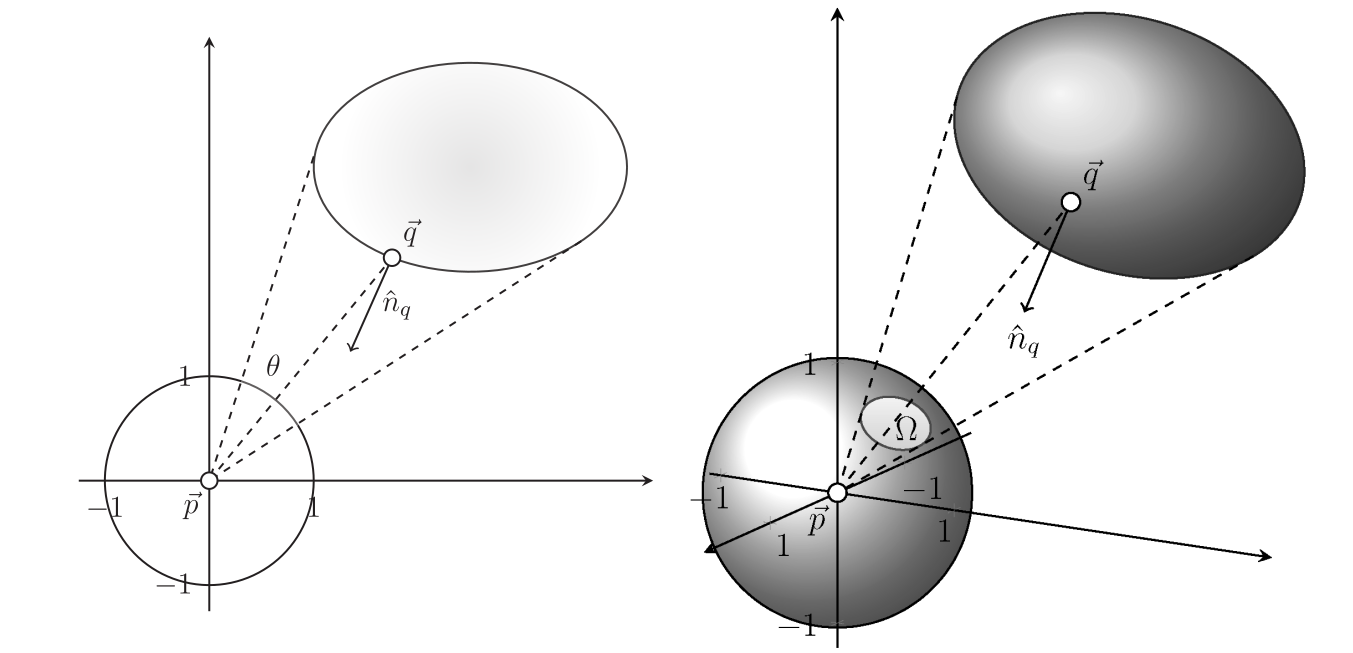
\includegraphics[width=\linewidth]{../assets/chapter3_surface_angle2area.png}
	\caption{Illustrazione dell'angolo (a sinistra) e angolo solido (a destra) sottesi da un punto dalla superficie visibile di un oggetto arbitrario.
		Immagine da \cite{pegoraro}}
	\label{chapter3:surface:angle2area}
\end{figure}
Come meglio spiegato in seguito (Capitolo \ref{chapter8}), Equazione \ref{chapter3:surface:renderingEq} \`e complessa anche perch\`e la relazione tra 
gli oggetti nella scena \`e implicita, incapsulata nella ray tracing function $t(\vec{p}, \hat{\omega})$. Una forma pi\`u trattabile di tale equazione
integrale la si pu\`o trovare trasformando l'integrale su un angolo solido in un integrale su un \textit{area} (vedi Figura 
\ref{chapter3:surface:angle2area}). L'angolo solido sotteso da un oggetto ad un punto $\vec{p}$ \`e una misura di \textit{area proiettata}, di una 
superficie parte di un oggetto visibile da $\vec{p}$, sulla sfera unitaria centrata in $\vec{p}$, ed \`e funzione sia dell'orientamento della normale 
della superficie osservata $\hat{n}_q$ ad ogni punto $\vec{q}=\vec{p}+\norm{\vec{q}-\vec{p}}\hat{\omega}=t((\vec{p}, \hat{\omega}_i),-\hat{\omega}_i)$, 
tale che $\hat{pq}=\hat{\omega}$, e sia della sua distanza da $\vec{p}$. Per esprimere tale relazione per ogni direzione dello spazio, definiamo 
$V(\vec{p},\vec{q})$ funzione di visibilit\`a binaria tra $\vec{p}$ e $\vec{q}$, tale che $V(\vec{p},\vec{q})=1$ se $\vec{q}$ appartiene all'insieme 
di superfici visibili da $\vec{p}$, e $V(\vec{p},\vec{q})=0$ se $\vec{p}$ e $\vec{q}$ sono mutualmente occlusi. Calcolare tale area proiettata consiste
nel proiettare ciascun elemento di superficie su una sfera di raggio $\norm{\vec{q}-\vec{p}}$ moltiplicando per il coseno dell'angolo formato tra la 
congiungente $\vec{p}$ a $\vec{q}$, e la normale $\hat{n}_q$, e dividere per il quadrato dell'area della sfera, in accordo con la definizione di 
angolo solido
\begin{equation}
	\mathrm{d}\hat{\omega}=\frac{V(\vec{p},\vec{q})}{\norm{\vec{p}-\vec{q}}^2}\langle\hat{n}_q,-\hat{pq}\rangle\mathrm{d}A(\vec{q})
\end{equation}
Tale relazione ricavata consiste nel jacobiano da utilizzare nell'integrale \ref{chapter3:surface:renderingEq} per la sostituzione delle variabili.
Inoltre, definiamo il Termine Geometrico $G(\vec{p},\vec{q})$, aggiungendo ai fattori della precedente formula il coseno dell'angolo tra direzione 
congiungente e $\hat{n}_p$, effettivamente proiettando angolo solido $\mathrm{d}\hat{\omega}$ sul piano equatoriale della sfera unitaria
centrata in $\vec{p}$
\begin{equation}\label{chapter3:surface:geometricTerm}
	G(\vec{p},\vec{q}) = \langle\hat{n}_p,\hat{pq}\rangle\frac{V(\vec{p},\vec{q})}{\norm{\vec{p}-\vec{q}}^2}\langle\hat{n}_q,-\hat{pq}\rangle
\end{equation}
tale che
\begin{equation}
	\langle\hat{n}_p,\hat{\omega}\rangle\mathrm{d}\hat{\omega} = %
		\langle\hat{n}_p,\hat{pq}\rangle\frac{V(\vec{p},\vec{q})}{\norm{\vec{p}-\vec{q}}^2}\langle\hat{n}_q,-\hat{pq}\rangle = %
		G(\vec{p},\vec{q})\mathrm{d}A(\vec{q})
\end{equation}
Possiamo dunque riformulare la Rendering Equation per essere un integrale nell'area dell'unione di tutte le superfici visibili dal punto $\vec{p}$
\begin{equation}
	L_o(\vec{p},\hat{pq}) %
		= L_e(\vec{p},\hat{pq}) + \int_{A}f_s(\vec{p},\hat{\omega}_o,\hat{pq})G(\vec{p},\vec{q})L_o(\vec{q},-\hat{pq})\mathrm{d}A(\vec{q})
\end{equation}
Torneremo in seguito su tale argomento.
\subsection{Modelli di BRDF}
Modelli di BRDFs derivano da diverse fonti, in particolare possono essere da dati misurati in laboratorio, da una simulazione di particelle, o da 
modelli analitici. Concentrandoci su questi ultimi, riusciamo ad individuare ulteriori suddivisioni basate sui fondamenti fisici di tali modelli
\begin{itemize}[topsep=0pt, noitemsep]
	\item \textit{Modelli Fenomenologici}: Equazioni che cercano di mimare determinati effetti osservabili senza alcun fondamento fisico preciso
	\item \textit{Turbid Models}: Equazioni che partono dal presupposto che tutti i fenomeni di subsurface light transport avvengano in scala
		microscopica, e applicano le equaizoni di Radiative Transfer Theory per derivare BRDF
	\item \textit{Modelli a Microcilindri}: Equazioni che modellano una superficie come composta da una collezione di cavit\`a cilindriche
	\item \textit{Modelli a Microgeometry}: Equazioni che modellano una superficie come composta da una collezione di facce planari microscopiche.
		Ci concentriamo su quest'ultima categoria
\end{itemize}
Come si osserva dall'Equazione \ref{chapter3:surface:reflectanceEq}, necessitiamo di strategie per campionare punti della funzione integranda per 
date direzioni $\hat{\omega}_i$, affinch\`e si assicuri una buona convergenza allo Stimatore di Monte Carlo per integrale\footnotemark{}. 
Una delle strategie proposte ed approfondite in seguito, \`e quella di campionare la funzione integranda con densit\`a di probabilit\`a $p$ 
proporzionale alla BRDF
\footnotetext{Tecnica nota come \textit{Importance Sampling}, approfondita in seguito}
\begin{equation}
	p(\vec{p},\hat{\omega}_o,\hat{\omega}_i) = \frac{f_s(\vec{p},\hat{\omega}_o,\hat{\omega}_i)\vert\langle\hat{n},\hat{\omega}_i\rangle\vert}%
		{\bar{\rho}(\vec{p},\hat{\omega}_o)}
\end{equation}
Dunque, assumendo di poter campionare da una distribuzione uniforme una osservazione della variabile aleatoria $\xi\sim\mathcal{U}(0,1)$, la cui 
implementazione si rimanda a Appendice \ref{appendixC}, analizziamo come poter trasformare tale variabile aleatoria per poter campionare con PDF 
proporzionale alla BRDF.\par
Analizziamo dunque due modelli fenomenologici, per poi passare a quelli basati su microgeometry
\subsubsection{Lambertian BRDF}
Ricordando l'equazione per \textit{Hemispherical-Directional Reflectance} (Equazione \ref{chapter3:surface:DHR}), supponiamo che la BRDF sia costante
nel dominio di integrazione, ovvero che la superficie sia lambertiana rispetto alla riflessione e opaca\footnotemark{}, producendo riflessione diffusa
perfetta.
\footnotetext{Inoltre, come sempre, ci limitiamo a considerare, con l'ottica geometrica, superfici solamente a livello dell'interfaccia}
\begin{figure}[tb]
	\centering
	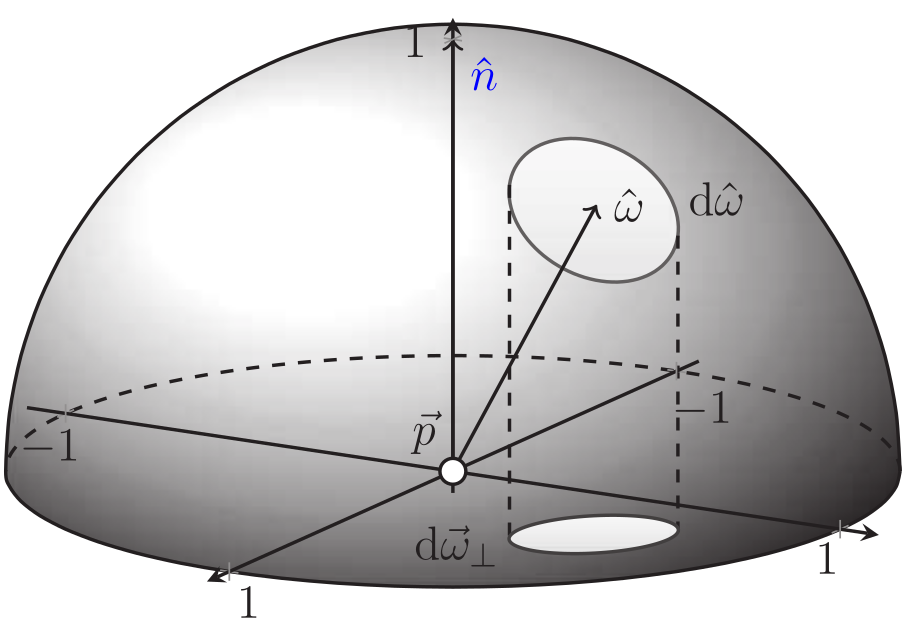
\includegraphics[width=0.8\linewidth]{../assets/chapter3_surface_projected_area.png}
	\caption{Illustrazione dell'area proiettata dell'emisfera secondo l'equazione 
		\mbox{$\mathrm{d}\hat{\omega}_\perp=\langle\hat{n},\hat{\omega}\rangle\mathrm{d}\hat{\omega}$}. Figura da \cite{pegoraro}}
	\label{chapter3:surface:projectedArea}
\end{figure}
\begin{equation}
	\rho(\vec{p},\hat{\omega}_o) = f_r(\vec{p})\int_{\mathcal{H}^2(\hat{n})}\vert\langle\hat{n},\hat{\omega}_i\rangle\vert\mathrm{d}\hat{\omega}_i%
		= f_r(\vec{p})\pi = \rho(\vec{p})
\end{equation}
da cui
\begin{equation}
	f_r(\vec{p}) = \frac{\rho(\vec{p})}{\pi}
\end{equation}
Il campionamento di tale BRDF pu\`o essere compiuto estraendo una direzione casuale nell'emisfera proiettata (vedi Figura 
\ref{chapter3:surface:projectedArea}). Tale proiezione \`e compiuta in quanto la BRDF \`e semplice, ed \`e moltiplicata per tale coseno. La PDF in
questione \`e la seguente: Siano $\hat{\omega}_z$ direzione dello zenith, $\hat{\omega}_i$ direzione incidente, la \textit{Cosine-lobe distribution} 
centrata attorno alla direzione dello zenith, con ripidit\`a $n$, \`e
\begin{equation}
	c_n(\omega_z) = \frac{n+1}{2\pi}\langle\hat{\omega}_z,\hat{\omega}_i\rangle^n
\end{equation}
Applichiamo la tecnica di \textit{Inverse Transform Sampling}, che, come approfondito in seguito (Capitolo \ref{chapter6}), permette di trasformare
una realizzazione campionata con una data PDF (nel nostro caso, $\mathcal{U}(0,1)$) ad una arbitraria, per la quale bisogna per\`o essere in grado di 
calcolare analiticamente la CDF ed invertirla. Per distribuzioni multivariate, tale tecnica \`e applicabile esclusivamente se la CDF \`e 
\textit{separabile}.\par
L'integrale in un angolo solido $\Omega_i$ per la \textit{Cosine-Lobe Distribution} risulta essere separabile nella forma
\begin{align}
	\int_{\Omega_i}c_n(\hat{\omega}_z,\hat{\omega}_i)\mathrm{d}\hat{\omega}_i &= \int_0^{\varphi_i}\frac{1}{2\pi}\mathrm{d}\varphi%
		\int_{\cos\theta_i}^1(n+1)\mu^n\mathrm{d}\mu \nonumber \\ 
	&= \left[\frac{\varphi_i}{2\pi}\right]_{\varphi=0}^{\varphi_i}\left[\mu^{n+1}\right]_{\mu=\cos\theta_i}^1 \nonumber \\
	&= \frac{\varphi_i}{2\pi}\left(1-\cos^{n+1}\theta_i\right)
\end{align}
Applicando \textit{Inverse Transform Sampling} permette di compiere \textit{Importance Sampling} come
\begin{align}
	\xi_\varphi = \frac{\varphi_i}{2\pi} &\longrightarrow\varphi_i = 2\pi\xi_\varphi \\
	\xi_\theta = 1-\cos^{n+1}\theta_i &\longrightarrow\theta_i = \arccos\left(\sqrt[n+1]{1-\xi_\theta}\right)
\end{align}
Il che permette di ottenere le coordinate sferiche della direzione campionata. Dunque, nel caso della Lambertian BRDF, campioniamo secondo la PDF
\begin{equation}
	p(\vec{p},\hat{\omega}_o,\hat{\omega}_i) = c_1(\hat{n},\hat{\omega}_i)
\end{equation}
\subsubsection{Specular BDRF}
Possiamo derivare una BRDF per una superficie che mostra riflessione speculare imponendo la condizione\footnotemark{}
\footnotetext{Si noti che $F_r(\langle\hat{n},\hat{\omega}_i\rangle)=F_r(\langle\hat{n},\hat{\omega}_o\rangle)=$}
\begin{align}
	L_o(\vec{p},\hat{\omega}_o)&=\int_{\mathcal{H}^2(\hat{n})}f_r(\vec{p},\hat{\omega}_o,\hat{\omega}_i)%
		L_i(\vec{p},\hat{\omega}_i)\vert\langle\hat{n},\hat{\omega}_i\rangle\vert\mathrm{d}\hat{\omega}_i%
		\\&=\left\{\begin{aligned}
			&F_r(\cos\theta_r)L_i(\vec{p},\hat{\omega}_r)\;\;&\mathrm{se}\;\hat{\omega}_o=\uptau_r(\hat{n},\hat{\omega}_r)\\
			&0 &\mathrm{altrimenti}
		\end{aligned}\right.
\end{align}
La quale risulta essere evidente come una Distribuzione di dirac moltiplicata per un opportuno fattore\footnotemark{}
\footnotetext{Le distribuzioni di Dirac, sia per le superfici che per le sorgenti luminose, devono essere riconosciute e trattate in maniera differente
	nelle routines di sampling}
\begin{equation}
	f_r(\vec{p},\hat{\omega}_o,\hat{\omega}_i)=F_r(\langle\hat{n},\hat{\omega}_o\rangle)%
		\frac{\delta(\hat{\omega}_i-\hat{\omega}_r)}{\vert\langle\hat{n},\hat{\omega}_i\rangle\vert}
\end{equation}
dove $\hat{\omega}_r=\uptau_r(\hat{\hat{n},\omega}_o)$\par
Similmente, usando la legge di Snell, possiamo ricavare una specular BTDF, ricordando che per la conservazione dell'energia
\begin{equation}
	\frac{\mathrm{d}^2\Phi_t(\vec{p},\hat{\omega}_t)}{\mathrm{d}^2\Phi_i(\vec{p},\hat{\omega}_i} = %
		\frac{L_t(\vec{p},\hat{\omega}_t)\mathrm{d}A(\vec{p})\langle\hat{n},\hat{\omega}_t\rangle\mathrm{d}\hat{\omega}_t}%
		{L_i(\vec{p},\hat{\omega}_i)\mathrm{d}A(\vec{p})\langle\hat{n},\hat{\omega}_i\rangle\mathrm{d}\hat{\omega}_i}
\end{equation}
Possiamo calcolare il jacobiano $\mathrm{d}\hat{\omega}_t/\mathrm{d}\hat{\omega}_i$ mediante osservazioni geometriche e la legge di Snell
\begin{align}
	\frac{\mathrm{d}\hat{\omega}_t}{\mathrm{d}\hat{\omega}_i} &= %
		\frac{\sin\theta_t\mathrm{d}\theta_t\mathrm{d}\varphi_t}{\sin\theta_t\mathrm{d}\theta_i\mathrm{d}\varphi_i} \nonumber \\
	&= \frac{\sin\theta_t}{\sin\theta_i}\frac{\mathrm{d}\arcsin\left(\frac{\eta_i}{\eta_t}\sin\theta_i\right)}{\mathrm{d}\theta_t} \nonumber \\
	&= \frac{\eta_i}{\eta_t}\frac{\frac{\eta_i}{\eta_t}\cos\theta_i}{\sqrt{1-\frac{\eta_i^2}{\eta_t^2}\sin^2\theta_t}} \nonumber \\
	&= \frac{\eta_i^2}{\eta_t^2}\frac{\cos\theta_i}{\sqrt{1-\sin^2\theta_t}} \nonumber \\
	&= \frac{\eta_i^2}{\eta_t^2}\frac{\cos\theta_i}{\cos\theta_t}
\end{align}
da cui
\begin{equation}
	\frac{L_t(\vec{p},\hat{\omega}_t)\mathrm{d}A(\vec{p})\langle\hat{n},\hat{\omega}_t\rangle\mathrm{d}\hat{\omega}_t}%
	{L_i(\vec{p},\hat{\omega}_i)\mathrm{d}A(\vec{p})\langle\hat{n},\hat{\omega}_i\rangle\mathrm{d}\hat{\omega}_i} = %
	\frac{L_t(\vec{p},\hat{\omega}_t)\eta^2_i}{L_i(\vec{p},\hat{\omega}_i)\eta^2_t} = T_{\frac{\eta_t}{\eta_i}}(\cos\theta_i)
\end{equation}
Da quest'ultima relazione si pu\`o ricavare che la transmittance $\eta_i\rightarrow\eta_t$, notazione $T_{\frac{\eta_t}{\eta_i}}$, calcolata in 
$\cos\theta_i$\footnotemark{}, \`e uguale alla transmittance $T_{\frac{\eta_i}{\eta_t}}$ calcolata in $\cos\theta_o$
\footnotetext{$\cos\theta_i=\cos\theta_t$ se la condizione del delta di Dirac \`e soddisfatta}
Dunque la condizione
\begin{align}
	L_o(\vec{p},\hat{\omega}_o)&=\int_{\mathcal{H}^2(-\hat{n})}f_t(\vec{p},\hat{\omega}_o,\hat{\omega}_i)%
		L_i(\vec{p},\hat{\omega}_i)\vert\langle\hat{n},-\hat{\omega}_i\rangle\vert\mathrm{d}\hat{\omega}_i%
		\\&=\left\{\begin{aligned}
			&\frac{\eta^2_t}{\eta_i^2}T_{\frac{\eta_i}{\eta_t}}(\langle\hat{n},\hat{\omega}_o\rangle)L_i(\vec{p},\hat{\omega}_t)%
				\;\;&\mathrm{se}\;\hat{\omega}_o=\uptau_t(\hat{n},\hat{\omega}_t)\\
			&0 &\mathrm{altrimenti}
		\end{aligned}\right.
\end{align}
dove $T_{\frac{\eta_i}{\eta_t}}(\langle\hat{n},\hat{\omega}_o\rangle)=T_{\frac{\eta_t}{\eta_i}}(\langle\hat{n},\hat{\omega}_i\rangle)%
	= 1 - F_r(\langle\hat{n},\hat{\omega}_i\rangle) = 1 - F_r(\langle\hat{n},\hat{\omega}_o\rangle)$
Da cui, con ragionamento analogo al precedente, si pu\`o ricavare la BTDF come delta di Dirac
\begin{equation}
	f_t(\vec{p},\hat{\omega}_o,\hat{\omega}_i)=T_{\frac{\eta_i}{\eta_t}}\frac{\eta_t^2}{\eta_i^2}(\vert\langle\hat{n},\hat{\omega}_o\rangle\vert)%
		\frac{\delta(\hat{\omega}_i-\hat{\omega}_t)}{-\vert\langle\hat{n},\hat{\omega}_i\rangle\vert}
\end{equation}
dove $\hat{\omega}_t=\uptau(\hat{n},\hat{\omega}_o)$\par
Il campionamento di tali BSDFs \`e gestito in modo speciale, in quanto solo se la PDF di campionamento \`e anch'essa una distribuzione di Dirac, 
con picco nella stessa posizione, allora la sampling routine ritorna un valore non nullo.
\subsection{Modelli di superficie secondo Microfacet Theory}
La \textit{Microfacet Theory} \`e un approccio basato sull'ottica geometrica che modella una superficie, come una collezione di facce planari
microscopiche, tipicamente con riflessione/trasmissione speculare (eccetto per il modello di Oren-Nayar, come si vedr\`a tra poco).\par
Affinch\`e l'assunzione di ottica geometrica sia valida, queste micro asperit\`a sono assunte molto pi\`u piccole (o molto pi\`u grandi) di una 
lunghezza d'onda. Una BRDF ricavata con tale teoria \`e un modello modellante lo scattering della luce in una grande collezione di microfacets con 
un \textit{approccio probabilistico}. Tale caratterizzazione \`e compicata dalle interazioni tra i microfacets illustrate in Figura 
\ref{chapter3:surface:microgeometryEffects}\par
\begin{figure}[tb]
	\centering
	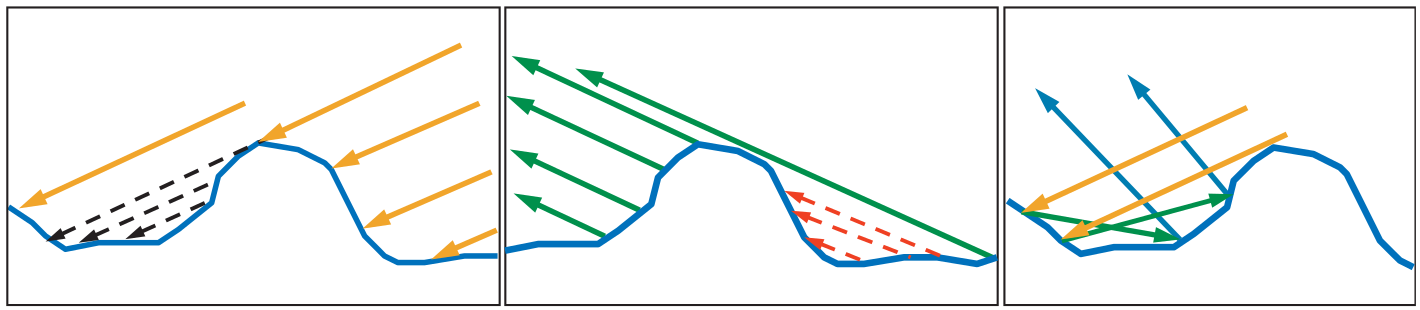
\includegraphics[width=\linewidth]{../assets/chapter3_surface_microgeometry_effectsAM.png}
	\caption{Illustrazione dei tre effetti di interazione tra microfacets e radiazione incidente. A sinistra, \textit{Shadowing}, per il quale 
		alcuni microfacets sono occlusi rispetto alla luce incidente da altri microfacets. Al centro, l'effetto complementare, \textit{Masking},
		per il quale alcuni microfacets sono occlusi rispetto all'osservatore da un altri microfacets. A destra, \textit{Interreflection}, per il
		quale luce incidente pu\`o "rimbalzare" su diversi microfacets prima di raggiungere l'osservatore. Questi tre effetti complicano la 
		definizione di una BRDF. Immagine da \cite{akenine-moller}}
	\label{chapter3:surface:microgeometryEffects}
\end{figure}
Un elemento di area della superficie $\mathrm{d}A$ \`e composto da un gran numero di microfacets, ciascuno di essi con la propria normale $\hat{m}$.
Possiamo caratterizzare tali normali come distribuite secondo una PDF proporzionale alla cosiddetta \textit{Normal Distribution Function} (NDF) 
$D(\vec{p},\hat{m})\geq0$. Maggiore \`e la varianza di tale distribuzione pi\`u la superficie \`e "rough". Per l'interazione dell'
\textit{Interreflection}, la luce pu\`o rimbalzare diverse volte prima di giungere all'osservatore, e tale contributo assume significativit\`a 
diversa a seconda della categoria del materiale \cite{akenine-moller}
\begin{itemize}[topsep=0pt,noitemsep]
	\item \textit{Dielettrici}: Contributi da riflessioni multiple sono man mano meno significativi per via del loro medio/basso Fresnel factor 
		(reflectance)
	\item \textit{Conduttori}: Il colore mostra i suoi maggior contributi nei rimbalzi successivi, in quanto alta reflectance e alto coefficiente di 
		assorbimento wavelength-selective fa si che nei rimbalzi multipli la luce assume una polarizzazione e shift del colore pi\`u significativi
\end{itemize}
Inoltre, ciascun materiale reagisce differentemente alla penetrazione da parte della luce nella superficie dando luogo a \textit{subsurface scattering}
di diversa intensit\`a. Nel caso in cui i microfacets sono molto pi\`u piccoli della lunghezza d'onda, possiamo approssimare affermando che la 
luce \`e uscita tutta nello stesso punto da cui \`e entrata, assunzione non precisa ma necessaria per usufruire del nostro modello di BRDF.\par
Ogni microfacet di normale $\hat{m}$, possiede anche una sua \textit{Micro BRDF} $f_\mu(\hat{m},\hat{\omega}_o,\hat{\omega}_i)$, i cui contributi sono
cumulati per ottenere la BRDF.\par
\begin{figure}
	\centering
	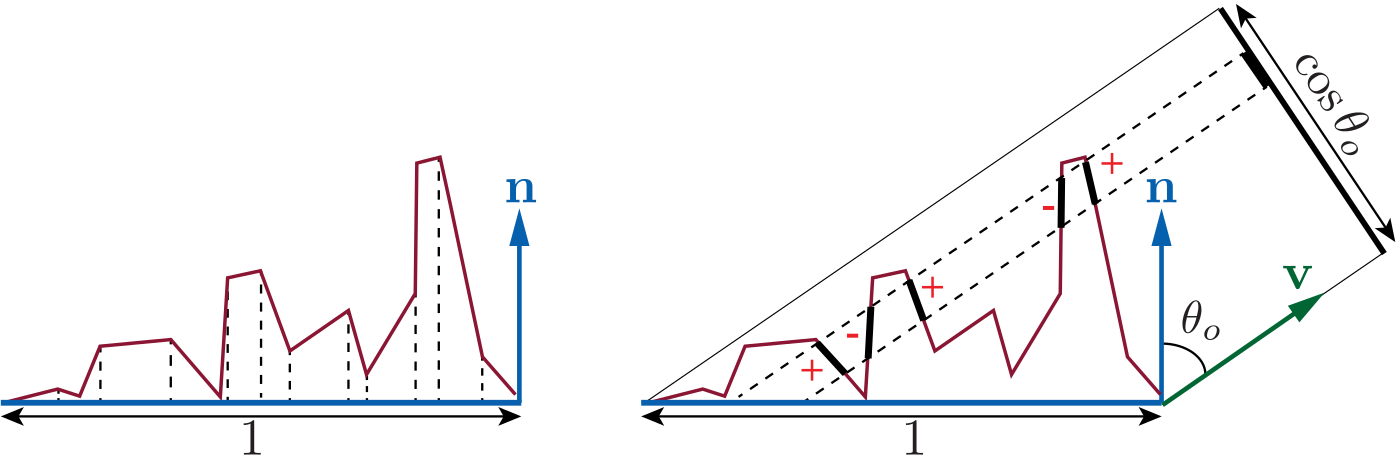
\includegraphics[width=\linewidth]{../assets/chapter3_surface_microgeometry_areaAM.png}
	\caption{Illustrazione del significato della Normal Distribution Function. Nota a destra, che nell'integrale della NDF proiettato, i contributi 
	occlusi si presentano sempre in coppia, uguali e con segno opposto, dunque non contribuiscono all'integrale. Immagine da \cite{akenine-moller}}
	\label{chapter3:surface:microgeometryArea}
\end{figure}
La \textit{Normal Distribution Function}, per convenzione, ha integrale pari al rapporto tra area della microsuperficie e macrosuperficie
\begin{equation}
	\int_{\mathcal{S}^2}D(\vec{p},\hat{m})\mathrm{d}\hat{m} = \frac{A_m}{A_n}\geq1
\end{equation}
Inoltre, nel caso tipico in cui la NDF sia un \textit{Height Field}, cio\`e 
\begin{equation}
	D(\vec{p},\hat{m})=0,\;\;\forall\hat{m}\,\vert\,\langle\hat{n},\hat{m}\rangle\leq0
\end{equation}
Allora l'area proiettata sulla macrosuperficie \`e unitaria
\begin{equation}
	\int_{\mathcal{H}^2(\hat{n})}D(\vec{p},\hat{m})\langle\hat{n},\hat{m}\rangle\mathrm{d}\hat{m}=1
\end{equation}
Pi\`u in generale, l'area della microsuperficie proiettata su un piano perpendicolare ad una direzione $\hat{\omega}$ 
(tipicamente quella dell'osservatore), pari all'\textit{area con segno} della microsuperficie (Figura \ref{chapter3:surface:microgeometryArea}) 
diviso l'area della macrosuperficie, \`e pari al coseno dell'angolo tra direzione e normale della macrosuperficie
\begin{equation}
	\int_{\mathcal{H}^2(\hat{n}}D(\vec{p},\hat{m})\langle\hat{\omega},\hat{m}\rangle\mathrm{d}\hat{m}=\langle\hat{n},\hat{\omega}\rangle
\end{equation}
I \textit{Masked} microfacets sono contributi che si semplificano nell'integrale, dunque esso \`e pari all'integrale dei \textit{microfacets visibili}.
Possiamo modellare ci\`o matematicamente definendo una \textit{Masking Function} o \textit{Mono-Static Visibility Function} (MVF), la quale, data 
normale microscopica $\hat{m}$ e direzione $\hat{\omega}$, definisce la percentuale aggregata di area di tutti i microfacets con normale $\hat{m}$,
visibile da $\hat{\omega}$, fratto l'area aggregata totale di tutti i microfacets con normale $\hat{m}$. Essa rappresenta dunque la 
\textit{probabilit\`a} di un microfacet con normale $\hat{m}$ di essere visibile da $\hat{\omega}$, 
\begin{equation}
	G_1(\vec{p},\hat{m},\hat{\omega}) = \Pr(\hat{\omega})
\end{equation}
Tale funzione $\in[0,1]$ e $G_1(\vec{p},\hat{m},\hat{\omega})=0,\,\mathrm{se}\,%
	\langle\hat{n},\hat{\omega}\rangle\langle\hat{m},\hat{\omega}\rangle\leq0$\par
Dunque, per definizione, $G_1(\vec{p},\hat{m},\hat{\omega}_o)D(\vec{p},\hat{\omega}_o)$ \`e la distribuzione dei microfacets visibili, tale che
\begin{equation}
	\int_{\mathcal{H}^2(\hat{n})}G_1(\vec{p},\hat{m},\hat{\omega}_o)D(\vec{p},\hat{m})\langle\hat{m},\hat{\omega}_o\rangle^+\mathrm{d}\hat{m}%
		=\langle\hat{n},\hat{\omega}_o\rangle
\end{equation}
dove $x^+=\max(0,x)$\par
Anche la funzione per modellare lo \textit{shadowing} \`e una \textit{Mono-Static Visibility Function}, infatti gode delle stesse propriet\`a della 
Masking Function, sostituendo $\hat{\omega}_i$ ad $\hat{\omega}_o$. Queste due funzioni sono combinate in qualche modo per ottenere la cosiddetta
\textit{Joint Shadowing-Masking Function} o \textit{Bi-Static Visibility Function} (BVF) $G_2$, definita come percentuale di area aggregata di 
microfacets con normale $\hat{m}$ simultaneamente visibile dalle due direzioni $\hat{\omega}_o$ e $\hat{\omega}_i$, fratto l'area totale di tutti i 
microfacets con normale $\hat{m}$. In termini di probabilit\`a,
\begin{equation}
	G_2(\vec{p},\hat{m},\hat{\omega}_o,\hat{\omega}_i) = \Pr(\hat{\omega}_o\cap\hat{\omega}_i)
\end{equation}
Se si assume che shadowing e masking sono incorrelati, il che pu\`o essere buona approssimazione solo per direzioni con differenza di angolo azimuthale
considerevole, allora
\begin{equation}
	G_2(\vec{p},\hat{m},\hat{\omega}_o,\hat{\omega}_i)=\Pr(\hat{\omega}_o)\Pr(\hat{\omega}_i)=%
		G_1(\vec{p},\hat{m},\hat{\omega}_o)G_1(\vec{p},\hat{m},\hat{\omega}_i)
\end{equation}
il che tende a provocare over darkening della superficie\footnote{infatti se $\hat{\omega}_o=\hat{\omega}_i$, allora dovremmo ottenere $G_1$. Invece,
con tale metodo, otteniamo $G_1^2$}
Per essere fisicamente plausibile, la probabilit\`a per un microfacet di essere visibile da due direzioni \`e minore, al pi\`u uguale se l'angolo 
azimuthale tra $\hat{\omega}_i$ e $\hat{\omega}_o$ \`e zero, a quella di essere visibile da una singola direzione
\begin{equation}
	G_2(\vec{p},\hat{m},\hat{\omega}_o,\hat{\omega}_i)\in[0, \min(G_1(\vec{p},\hat{m},\hat{\omega}_o),G_1(\vec{p},\hat{m},\hat{\omega}_i))]
\end{equation}
Inoltre la microstruttura \`e visibile solo dalla emisfera la cui normale macroscopica forma un angolo acuto, da entrambe le direzioni
\begin{equation}
	G_2(\vec{p},\hat{m},\hat{\omega}_o,\hat{\omega}_i) = 0,\;\;\mathrm{se}\,%
		\langle\hat{n},\hat{\omega}_o\rangle\langle\hat{m},\hat{\omega}_o\rangle\leq0%
		\langle\hat{n},\hat{\omega}_i\rangle\langle\hat{m},\hat{\omega}_i\rangle\leq0
\end{equation}
Infine soddisfa la propriet\`a di reciprocit\`a $G_2(\vec{p},\hat{m},\hat{\omega}_o,\hat{\omega}_i)=G_2(\vec{p},\hat{m},\hat{\omega}_i,\hat{\omega}_o)$.
\par
Analizziamo brevemente due modelli di visibilit\`a, la cui dimostrazione completa si rimanda a \cite{pegoraro}: \textit{V-Cavity Function} e
\textit{Smith's Visibility Function}.
